\section*{Database CLAY/10/7490 数据库CLAY/10/7490}

\begin{Parallel}{0.60\textwidth}{}
    \ParallelLText
    {
        This study compiles a clay database (CLAY/10/7490) from the literature consisting of a large number of data points. This database consists of data points from 251 studies. The number of data points associated with each study varies from 1 to 419 with an average 30 data points per study. The geographical regions cover Australia, Austria, Brazil, Canada, China, England, Finland, France, Germany, Hong Kong, India, Iraq, Italy, Japan, Korea, Malaysia, Mexico, New Zealand, Northern Ireland, Norway, Poland, Singapore, South Africa, Spain, Sweden, Taiwan, Thailand, United Kingdom, United States, and Venezuela. The clay properties cover a wide range of overconsolidation ratio (OCR) values (but mostly 1$\sim$10), a wide range of sensitivity (St) values (sites with St = 1~tens or hundreds are fairly typical), and a wide range of plasticity index (PI) values (but mostly 8$\sim$100). Figure 1 shows the plasticity chart and Robertson’s CPTU soil classification chart \citep{Robertson1990151} of all data points in the database — most data points are classified as clays (some are sensitive or organic clays). Some data points are classified as clayey silts or silt mixtures, and a few are classified as sand mixtures or sands. The details of this database are shown in Appendix \ref{appendix:a}.
    }
    \ParallelRText
    {
        这项研究从文献中汇编了一个包含大量数据点的粘土数据库(CLAY / 10/7490)。该数据库包含来自251个研究的数据点。与每个研究相关的数据点数量从1到419不等,每个研究平均30个数据点。地理区域包括澳大利亚,奥地利,巴西,加拿大,中国,英国,芬兰,法国,德国,香港,印度,伊拉克,意大利,日本,韩国,马来西亚,墨西哥,新西兰,北爱尔兰,挪威,波兰,新加坡,南非,西班牙,瑞典,台湾,泰国,英国,美国和委内瑞拉。黏土的特性涵盖了大范围的超固结比(OCR)值(但大多为1$\sim$10),大范围的敏感度(St)值($S_t$ = 1$\sim$数十或数百的值是相当典型的)和大范围的塑性指数(PI)值(但多数为8$\sim$100)。图\ref{figure:1}显示了数据库中所有数据点的可塑性图和Robertson的CPTU土壤分类图\citep{Robertson1990151}——大多数数据点被归类为黏土(一些是敏感黏土或有机黏土)。一些数据点被分类为黏土粉砂或粉砂混合物,而一些数据点被分类为砂混合物或砂。该数据库的详细信息显示在附录\ref{appendix:a}中。
    }
    \ParallelPar
    \begin{figure}[htb]
    \centering
    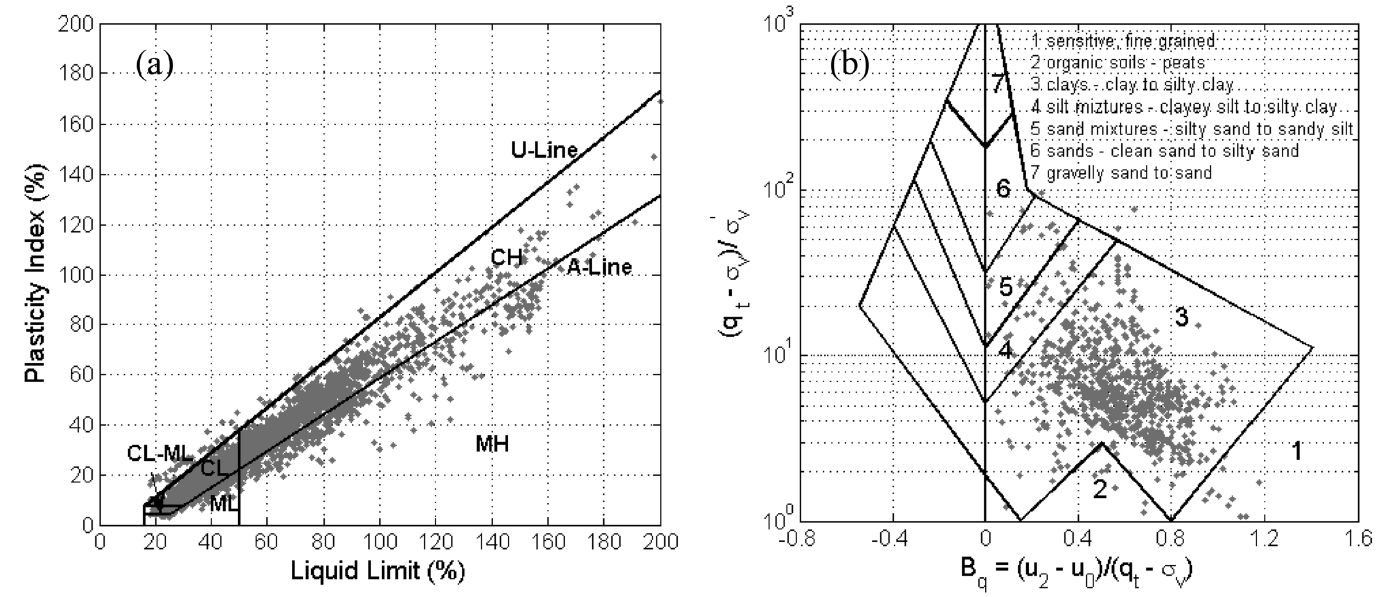
\includegraphics[width=0.8\textwidth]{figures/figure-1.png}
    \caption{(a) Plasticity chart; (b) \citet{Robertson1990151} CPTU soil classification chart. $B_q$, pore pressure ratio; CH, high-plasticity clay; CL, lowplasticity clay; MH, high-plasticity silt; ML, low-plasticity silt; $q_t$, corrected cone tip resistance; $u_0$, hydrostatic pore pressure; $u_2$, pore pressure behind the cone; $\sigma_v$, total effective stress; $\sigma_v'$, vertical effective stress.}
    \addtocounter{figure}{-1}
    \vspace{-5pt}
    \renewcommand{\figurename}{图}
    \caption{(a)可塑性图; (b)\citet{Robertson1990151}的CPTU土壤分类图。 $B_q$,孔隙压力比; CH,高塑性粘土; CL,低塑性粘土; MH,高塑性淤泥; ML,低塑性淤泥; $q_t$,校正的锥头电阻; $u_0$,静水孔隙压力; $u_2$,锥体后面的孔隙压力; $\sigma_v$,总有效应力; $\sigma_v'$,垂直有效应力。}
    \renewcommand{\figurename}{Figure}
    \label{figure:1}
\end{figure}
    \ParallelLText
    {
        Ten dimensionless parameters of clays are of primary interest. They are categorized into three groups:

        \textbf{1. Index properties,} including liquid limit (LL), plasticity index (PI), and liquidity index (LI). 

        \textbf{2. Stresses and strengths,} including normalized vertical effective stress ($\sigma_v'/P_a$, where $P_a$ is one atmosphere pressure (=101.3$\rm{kN/m^2}$)), normalized preconsolidation stress ($\sigma_p'/P_a$), normalized undrained shear strength ($s_u/\sigma_v'$), and sensitivity ($S_t=s_u/s_u^{re}$, where $s_u^{re}$ is the remoulded undrained shear strength). The $s_u$ values in the literature were obtained based on various types of tests, including isotropically consolidated undrained compression (CIUC), $K_0$-consolidated undrained compression (C$K_0$UC), $K_0$-consolidated undrained extension (C$K_0$UE), direct simple shear (DSS), unconsolidated undrained compression (UU), unconfined compression (UC), and field vane (FV). These values cannot be compared directly because $s_u$ depends on stress state, strain rate, and sampling disturbance. By following the recommendations made by \citet{Bjerrum19721}, \citet{Kulhawy1990}, and \citet{Mesri20071}, these $s_u$ values are all converted to the “mobilized” $s_u$ values, denoted by $s_u(\rm{mob})$, which is defined as the in situ undrained shear strength mobilized in embankment and slope failures \citep{Mesri20071}. The transformation models used to convert undrained shear strengths derived from different test types to the reference $s_u(\rm{mob})$ are given in Table \ref{table:2}. 

        \textbf{3. Parameters from the piezocone test (CPTU),} including pore pressure ratio $B_q=(u_2-u_0)/(q_t-\sigma_v)$, where $u_2$ is the pore pressure behind the cone, $u_0$ is the hydrostatic pore pressure, $q_t$ is the corrected cone tip resistance, and $\sigma_v$ is the total effective stress; normalized cone tip resistance $(q_t-\sigma_v)/\sigma_v'$ ; and normalized effective cone tip resistance $q_t-u_2/\sigma_v'$. \par
        The CPTU data are nearly continuous with depth. However, only a few data points in a CPTU profile are adopted into the database at the depths where other clay parameters (such as $s_u$ and PI) are also known. As a result, the vertical interval of the adopted CPTU data points at the same site is about 1 to 3 m. Note that the point data at the appropriate depths are adopted. A possible refinement involving averaging along the length of the undisturbed sample was not considered.
    }
    \ParallelRText
    {
        十个无量纲的黏土参数是最重要的。它们分为三类:

        \textbf{1. 指数性质,}包括液体极限(LL),可塑性指数(PI)和流动性指数(LI)。

        \textbf{2. 应力和强度,}包括归一化垂直有效应力($\sigma_v'/P_a$,其中$P_a$是一个大气压,归一化预固结应力($\sigma_p'/P_a$),归一化不排水剪切强度($s_u/\sigma_v'$)和灵敏度($S_t=s_u/s_u^{re}$,其中$s_u^{re}$是重新模制的不排水剪切强度)。文献中的$s_u$值是根据各种类型的测试获得的,包括各向同性固结不排水压缩(CIUC),$K_0$固结不排水压缩(C$K_0$UC),$K_0$固结不排水延伸(C$K_0$UE),直接简单剪切(DSS),未固结不排水压缩(UU),无限制压缩(UC)和现场叶片(FV)。这些值不能直接比较,因为$s_u$取决于应力状态,应变率和采样扰动。通过遵循\citet{Bjerrum19721},\citet{Kulhawy1990}以及\citet{Mesri20071}的建议,这些$s_u$值都被转换为“扰动” $s_u$值,该值由$s_u(\rm{mob})$定义,因为在路堤和边坡破坏中扰动了原地不排水的抗剪强度\citep{Mesri20071}。表\ref{table:2}给出了用于将源自不同测试类型的不排水剪切强度转换为参考$s_u(\rm{mob})$的转换模型。

        \textbf{3. 压电锥测试(CPTU)的参数,}包括孔隙压力比$B_q=(u_2-u_0)/(q_t-\sigma_v)$,其中$u_2$是圆锥体后面的孔隙压力,$u_0$是静水孔隙压力,$q_t$是校正的锥头阻力,$\sigma_v$是总有效应力;归一化锥头电阻$(q_t-\sigma_v)/\sigma_v'$;以及归一化的有效锥端电阻$q_t-u_2/\sigma_v'$。\par
        CPTU数据在深度上几乎是连续的。但是,在已知其他黏土参数(例如$s_u$和PI)的深度处,CPTU剖面中只有几个数据点被采用到数据库中。结果,在同一站点上采用的CPTU数据点的垂直间隔约为1至3 m。注意,采用了适当深度的点数据。没有考虑可能的改进,包括沿未扰动样本的长度取平均值。
    }
    \ParallelPar
    \begin{table}[!htb]
    \centering
    \scriptsize
    \caption{Transformation models for $s_u(\rm{mob})$.}
    \addtocounter{table}{-1}
    \vspace{-8pt}
    \renewcommand{\tablename}{表}
    \caption{$s_u(\rm{mob})$的转换模型}
    \vspace{4pt}
    \renewcommand{\tablename}{Table}
    \begin{tabularx}{\textwidth}{lll}
        \toprule
        Available $s_u$ information & Transformation model & Reference\\
        \midrule
        FV & $s_u(\rm{mob})\approx{}s_u(\rm{field})\approx{}[s_u(\rm{FV})]\mu$ & \citet{Bjerrum19721} \\
        UC & $s_u(\rm{mob})\approx{}s_u(\rm{UC})$ & \citet{Mesri20071} \\
        UU & $s_u(\rm{mob})/\sigma_v'\approx{}s_u(\rm{UC})/\sigma_v'\approx{}-0.073+1.018s_u(\rm{UU})/\sigma_v'$ & \citet{Chen19931732};\citet{Mesri20071} \\
        CIUC & $s_u(\rm{mob})/\sigma_v'\approx{}s_u(\rm{UC})/\sigma_v'\approx{}-0.278+1.172s_u(\rm{CIUC})/\sigma_v'$ & \citet{Chen19931732};\citet{Mesri20071} \\
        C$K_0$UC, DSS, C$K_0$UE & $s_u(\rm{mob})\approx{}\{[s_u(\rm{C}K_0\rm{UC})+s_u(\rm{DSS})+s_u(\rm{C}K_0\rm{UE})]/3\}\mu_t$ & \citet{Mesri20071};\citet{Kulhawy1990}\\
        C$K_0$UC, C$K_0$UE & $s_u(\rm{mob})\approx{}\{[s_u(\rm{C}K_0\rm{UC})+s_u(\rm{C}K_0\rm{UE})]/2\}\mu_t^*$ & \citet{Mesri20071};\citet{Kulhawy1990}\\
        DSS & $s_u(\rm{mob})\approx{}[s_u(\rm{DSS})]u_t^*$ & \citet{Mesri20071};\citet{Kulhawy1990}\\
        C$K_0$UC & $s_u(\rm{mob})\approx{}[s_u(\rm{DSS})]u_t\approx{}[s_u(\rm{C}K_0\rm{UC})][0.67\mu_t]$ & \citet{Mesri20071};\citet{Kulhawy1990}\\
        C$K_0$UE & $s_u(\rm{mob})\approx{}[s_u(\rm{DSS})]u_t\approx{}[s_u(\rm{C}K_0\rm{UE})][1.53^\dag(\mu_t)]$ & \citet{Mesri20071};\citet{Kulhawy1990}\\
        \bottomrule
    \end{tabularx}%
    {\raggedright\vspace{4pt}

    ~~~~\textbf{Note:} FV, field vane; UC, unconfined compression; UU, unconsolidated undrained compression; CIUC, isotropically consolidated undrained compression; C$K_0$UC, $K_0$-consolidated undrained compression; DSS, direct simple shear; C$K_0$UEE, $K_0$-consolidated undrained extension; $\mu$ , PI-dependent correction factor for $s_u(\rm{FV})$ proposed in \citet{Bjerrum19721}; $\mu_t$, PI-dependent strain rate correction factor proposed in \citet{Terzaghi1996}. 

    ~~~~*These equations are based on the following two facts: $(i) s_u(\rm{mob}\approx{}\{[s_u(\rm{C}K_0\rm{UC})+s_u(\rm{DSS})+s_u(\rm{C}K_0\rm{UC})]/3\}\mu_t$ and $(ii)s_u(\rm{DSS})$ is roughly the average of $s_u(\rm{C}K_0\rm{UC})$ and $s_u(\rm{C}K_0\rm{UE})$ \citep{Kulhawy1990}. 

    ~~~~$\dag$This constant of 1.53 is based on the following two facts: $(i)su(\rm{DSS})\approx{}0.67s_u(\rm{C}K_0\rm{UC})$\citep{Kulhawy1990} and $(ii) s_u(\rm{DSS})$ is roughly the average of $s_u(\rm{C}K_0\rm{UC})$ and $s_u(\rm{C}K_0\rm{UE})$.

    ~~~~\textbf{注意:} FV,现场试验; UC,无限制压缩; UU,不固结不排水压缩; CIUC,各向同性固结不排水压缩; C$K_0$UC,$K_0$固结不排水压缩; DSS,直接剪切; C$K_0$UE,$K_0$固结不排水拉伸;$\mu$,\citet{Bjerrum19721}提出的$s_u(\rm{FV})$的PI依赖校正因子;$\mu_t$,\citet{Terzaghi1996}提出的依赖PI的应变率校正因子。

    ~~~~*这些方程式基于以下两个事实:$(i) s_u(\rm{mob}\approx{}\{[s_u(\rm{C}K_0\rm{UC})+s_u(\rm{DSS})+s_u(\rm{C}K_0\rm{UC})]/3\}\mu_t$,$(ii)s_u(\rm{DSS})$大致为$s_u(\rm{C}K_0\rm{UC})$和$s_u(\rm{C}K_0\rm{UE})$的平均值\citep{Kulhawy1990}。

    ~~~~$\dag$1.53的常数基于以下两个事实:$(i)su(\rm{DSS})\approx{}0.67s_u(\rm{C}K_0\rm{UC})$\citep{Kulhawy1990},$(ii) s_u(\rm{DSS})$大约是$s_u(\rm{C}K_0\rm{UC})$和$s_u(\rm{C}K_0\rm{UE})$的平均值。

    }
    \label{table:2}%
\end{table}

    \ParallelLText
    {
        Some other dimensionless parameters of interest, such as $s_u/\sigma_p'$, OCR, and $s_u^{re}/P_a$, can be derived from the above 10 parameters. The basic statistics of all these parameters (10 basic parameters together with $s_u/\sigma_p'$, OCR, and $s_u^{re}/P_a$) are listed in Table \ref{table:3}. The numbers of available data points ($n$) are shown in the second column. The statistics are the mean value, coefficient of variation (COV), minimum value (min), and maximum value (max). Their percentiles are listed in Table \ref{table:4}, where the median values (50$\%$ percentiles) are shaded. It is worth mentioning that the statistical uncertainty is higher for the lower and higher percentiles.
    }
    \ParallelRText
    {
        可以从上述10个参数中得出其他一些无量纲的感兴趣参数,例如$s_u/\sigma_p'$,OCR和$s_u^{re}/P_a$。 表\ref{table:3}列出了所有这些参数的基本统计信息(连同$s_u/\sigma_p'$,OCR和$s_u^{re}/P_a$一起的10个基本参数)。第二列显示了可用数据点的数量($n$)。 统计信息是平均值,变异系数(COV),最小值(min)和最大值(max)。 表\ref{table:4}中列出了它们的百分位数,其中中值(50%百分数)用阴影表示。 值得一提的是,上下百分位数的统计不确定性较高。
    }
    \ParallelPar
    \begin{table}[!htb]
    \centering
    \begin{minipage}[t]{0.44\textwidth}
        \centering
        \scriptsize
        \caption{Statistics of the data points in the database.}
        \addtocounter{table}{-1}
        \vspace{-8pt}
        \renewcommand{\tablename}{表}
        \caption{数据库中数据点的统计信息。}
        \vspace{4pt}
        \renewcommand{\tablename}{Table}
        \begin{tabular}{llllll}
            \toprule
            Variable                    & $n$   & Mean  & COV   & Min     & Max\\
            \midrule
            LL                          & 3822  & 67.7  & 0.80  & 18.1    & 515 \\
            PI                          & 4265  & 39.7  & 1.08  & 1.9     & 363 \\
            LI                          & 3661  & 1.01  & 0.78  & -0.75   & 6.45 \\
            $\sigma_y'/P_a$             & 3370  & 1.8   & 1.47  & 4.13E-3 & 38.74 \\
            $\sigma_p'/P_a$             & 2028  & 4.37  & 2.31  & 0.094   & 193.3 \\
            $s_u/\sigma_v'$             & 3532  & 0.51  & 1.25  & 3.68E-3 & 7.78 \\
            $S_t$                       & 1589  & 35.0  & 2.88  & 1.0     & 1467 \\
            $B_q$                       & 1016  & 0.58  & 0.35  & 0.01    & 1.17 \\
            $(q_t-\sigma_v)/\sigma_v'$  & 862   & 8.9   & 1.17  & 0.48    & 95.98 \\
            $(q_t-u_2)/\sigma_v'$       & 668   & 5.34  & 1.37  & 0.61    & 108.2 \\
            $s_u/\sigma_p'$             & 1467  & 0.23  & 0.55  & 3.68E-3 & 1.34 \\
            OCR                         & 3531  & 3.85  & 1.56  & 1.0     & 60.23 \\
            $s_u^{re}/P_a$              & 1143  & 0.075 & 2.86  & 9.67E-5 & 2.47 \\
            \bottomrule
        \end{tabular}%
        \label{table:3}%
    \end{minipage}
    \begin{minipage}[t]{0.55\textwidth}
        \centering
        \scriptsize
        \caption{Statistics of the data points in the database.}
        \addtocounter{table}{-1}
        \vspace{-8pt}
        \renewcommand{\tablename}{表}
        \caption{数据库中数据点的统计信息。}
        \vspace{4pt}
        \renewcommand{\tablename}{Table}
        \begin{tabular}{llll>{\columncolor{gray}}llll}
            \toprule
            Variable & $2.5\%$ & $5\%$ & $25\%$ & $50\%$ & $75\%$ & $95\%$ & $97.5\%$\\
            \midrule
            LL                          &  23.6    & 26.2      & 39.0      & 54.3  & 76    & 149.1 & 200.0 \\
            PI                          &  5.8     & 8.0       & 18.5      & 29.3  & 46    & 91.4  & 135.0 \\
            LI                          &  -8.6E-2 & 4.7E-3    & 0.54      & 0.87  & 1.32  & 2.51  & 3.0 \\
            $\sigma_y'/P_a$             &  0.11    & 0.14      & 0.43      & 0.94  & 2.03  & 6.27  & 8.37 \\
            $\sigma_p'/P_a$             &  0.26    & 0.33      & 0.8       & 1.71  & 3.69  & 19.57 & 29.19 \\
            $s_u/\sigma_v'$             &  0.08    & 0.11      & 0.21      & 0.31  & 0.56  & 1.46  & 2.25 \\
            $S_t$                       &  1.7     & 2.3       & 5.0       & 8.0   & 23.0  & 140.8 & 217.6 \\
            $B_q$                       &  0.15    & 0.23      & 0.45      & 0.57  & 0.72  & 0.91  & 0.99 \\
            $(q_t-\sigma_v)/\sigma_v'$  &  1.92    & 2.43      & 4.15      & 5.79  & 8.77  & 27.57 & 44.07 \\
            $(q_t-u_2)/\sigma_v'$       &  1.28    & 1.51      & 2.42      & 3.63  & 5.67  & 14.97 & 18.55 \\
            $s_u/\sigma_p'$             &  6.30E-2 & 8.38E-2   & 0.15      & 0.21  & 0.27  & 0.44  & 0.56 \\
            OCR                         &  1.0     & 1.0       & 1.04      & 1.73  & 3.57  & 15.79 & 24.00 \\
            $s_u^{re}/P_a$              &  5.14E-4 & 8.05E-4   & 6.48E–3   & 0.021 & 0.062 & 0.26 &  0.54 \\
            
            \bottomrule
        \end{tabular}%
        \label{table:4}%
    \end{minipage}
\end{table}

\end{Parallel}
